\documentclass[tikz, crop, border = {2pt 2pt 2pt 2pt}]{standalone}

\usetikzlibrary{decorations.pathreplacing, decorations.text, calc}
\usepackage{physics}
\usepackage{concmath-otf}

\begin{document}
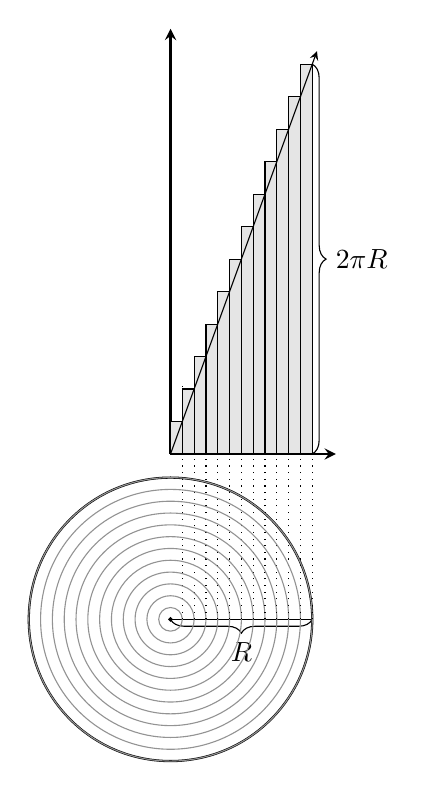
\begin{tikzpicture}[scale = 0.6]
    \draw[thick] (0, 0) circle (3);
    \filldraw (0, 0) circle (1pt);
    \draw (0, 0) -- (3, 0);
    \draw[decorate, decoration = {brace, amplitude = 5pt, mirror}] (0, 0) -- (3, 0) node[below = 5pt, midway]{$R$};
    \foreach \x in {0.25, 0.5, ..., 3}{
        \draw[gray!85] (0, 0) circle (\x);
        \draw[dotted] (\x, 0) -- ++ (0, 5);
    }

    \begin{scope}[shift = {(0, 3.5)}]
        \draw[thick, -stealth] (0, 0) -- (0, 9);
        \draw[thick, -stealth] (0, 0) -- (3.5, 0);

        \foreach \x in {0.25, 0.5, ..., 3}{
            \filldraw[fill = lightgray!40, draw = black] ({\x-0.25}, 0) rectangle ++ (0.25, {2.75*\x});
        }
        \draw[decorate, decoration = {brace, amplitude = 5pt, mirror}] (3, 0) -- ++ (0, {2.75*3}) node[right = 5pt, midway]{$2\pi R$};

        \draw[-stealth] (0, 0) -- ++ (3.1, {2.75*3.1});
    \end{scope}
\end{tikzpicture}
\end{document}